\section{问题四的建模与求解}

\subsection{相关性分析}

为了找出与术后满意度相关的特征,我们将以术后满意度为标签来计算各个特征的相关性,使用Spearman和Kendall相关性分析,Spearman相关系数公式已给出,介绍Kendall原理:

设有两个随机变量$\overrightarrow{X}=\left( {{x}_{1}},{{x}_{2}},...,{{x}_{n}} \right),\overrightarrow{Y}=\left( {{y}_{1}},{{y}_{2}},...,{{y}_{n}} \right)$,将它们分别排名得到两个的排名向量$\overrightarrow{X}=\left( {{r}_{1}},{{r}_{2}},...,r \right),\overrightarrow{Y}=\left( {{s}_{1}},{{s}_{2}},...,{{s}_{n}} \right)$,得到相关系数:

\begin{equation}
    \tau = \dfrac{2}{n(n-2)}\sum_{i=1}^{n-1}\sum_{j=i+1}^{n}\text{sgn}{(x_i-x_j)}\text{sgn}{(y_i-y_j)}.
\end{equation}
其中,表示$\text{sgn}(x)$的$x$符号系数,当$x>0$时,$\text{sgn}(x)=1$,当$x=0$时,$\text{sgn}(x)=0$,当$x<0$时,$\text{sgn}(x)=-1$。分别计算得到的相关性如下图所示:

\begin{figure}[H] % 这个H不要动!
	\centering % 不要动!
	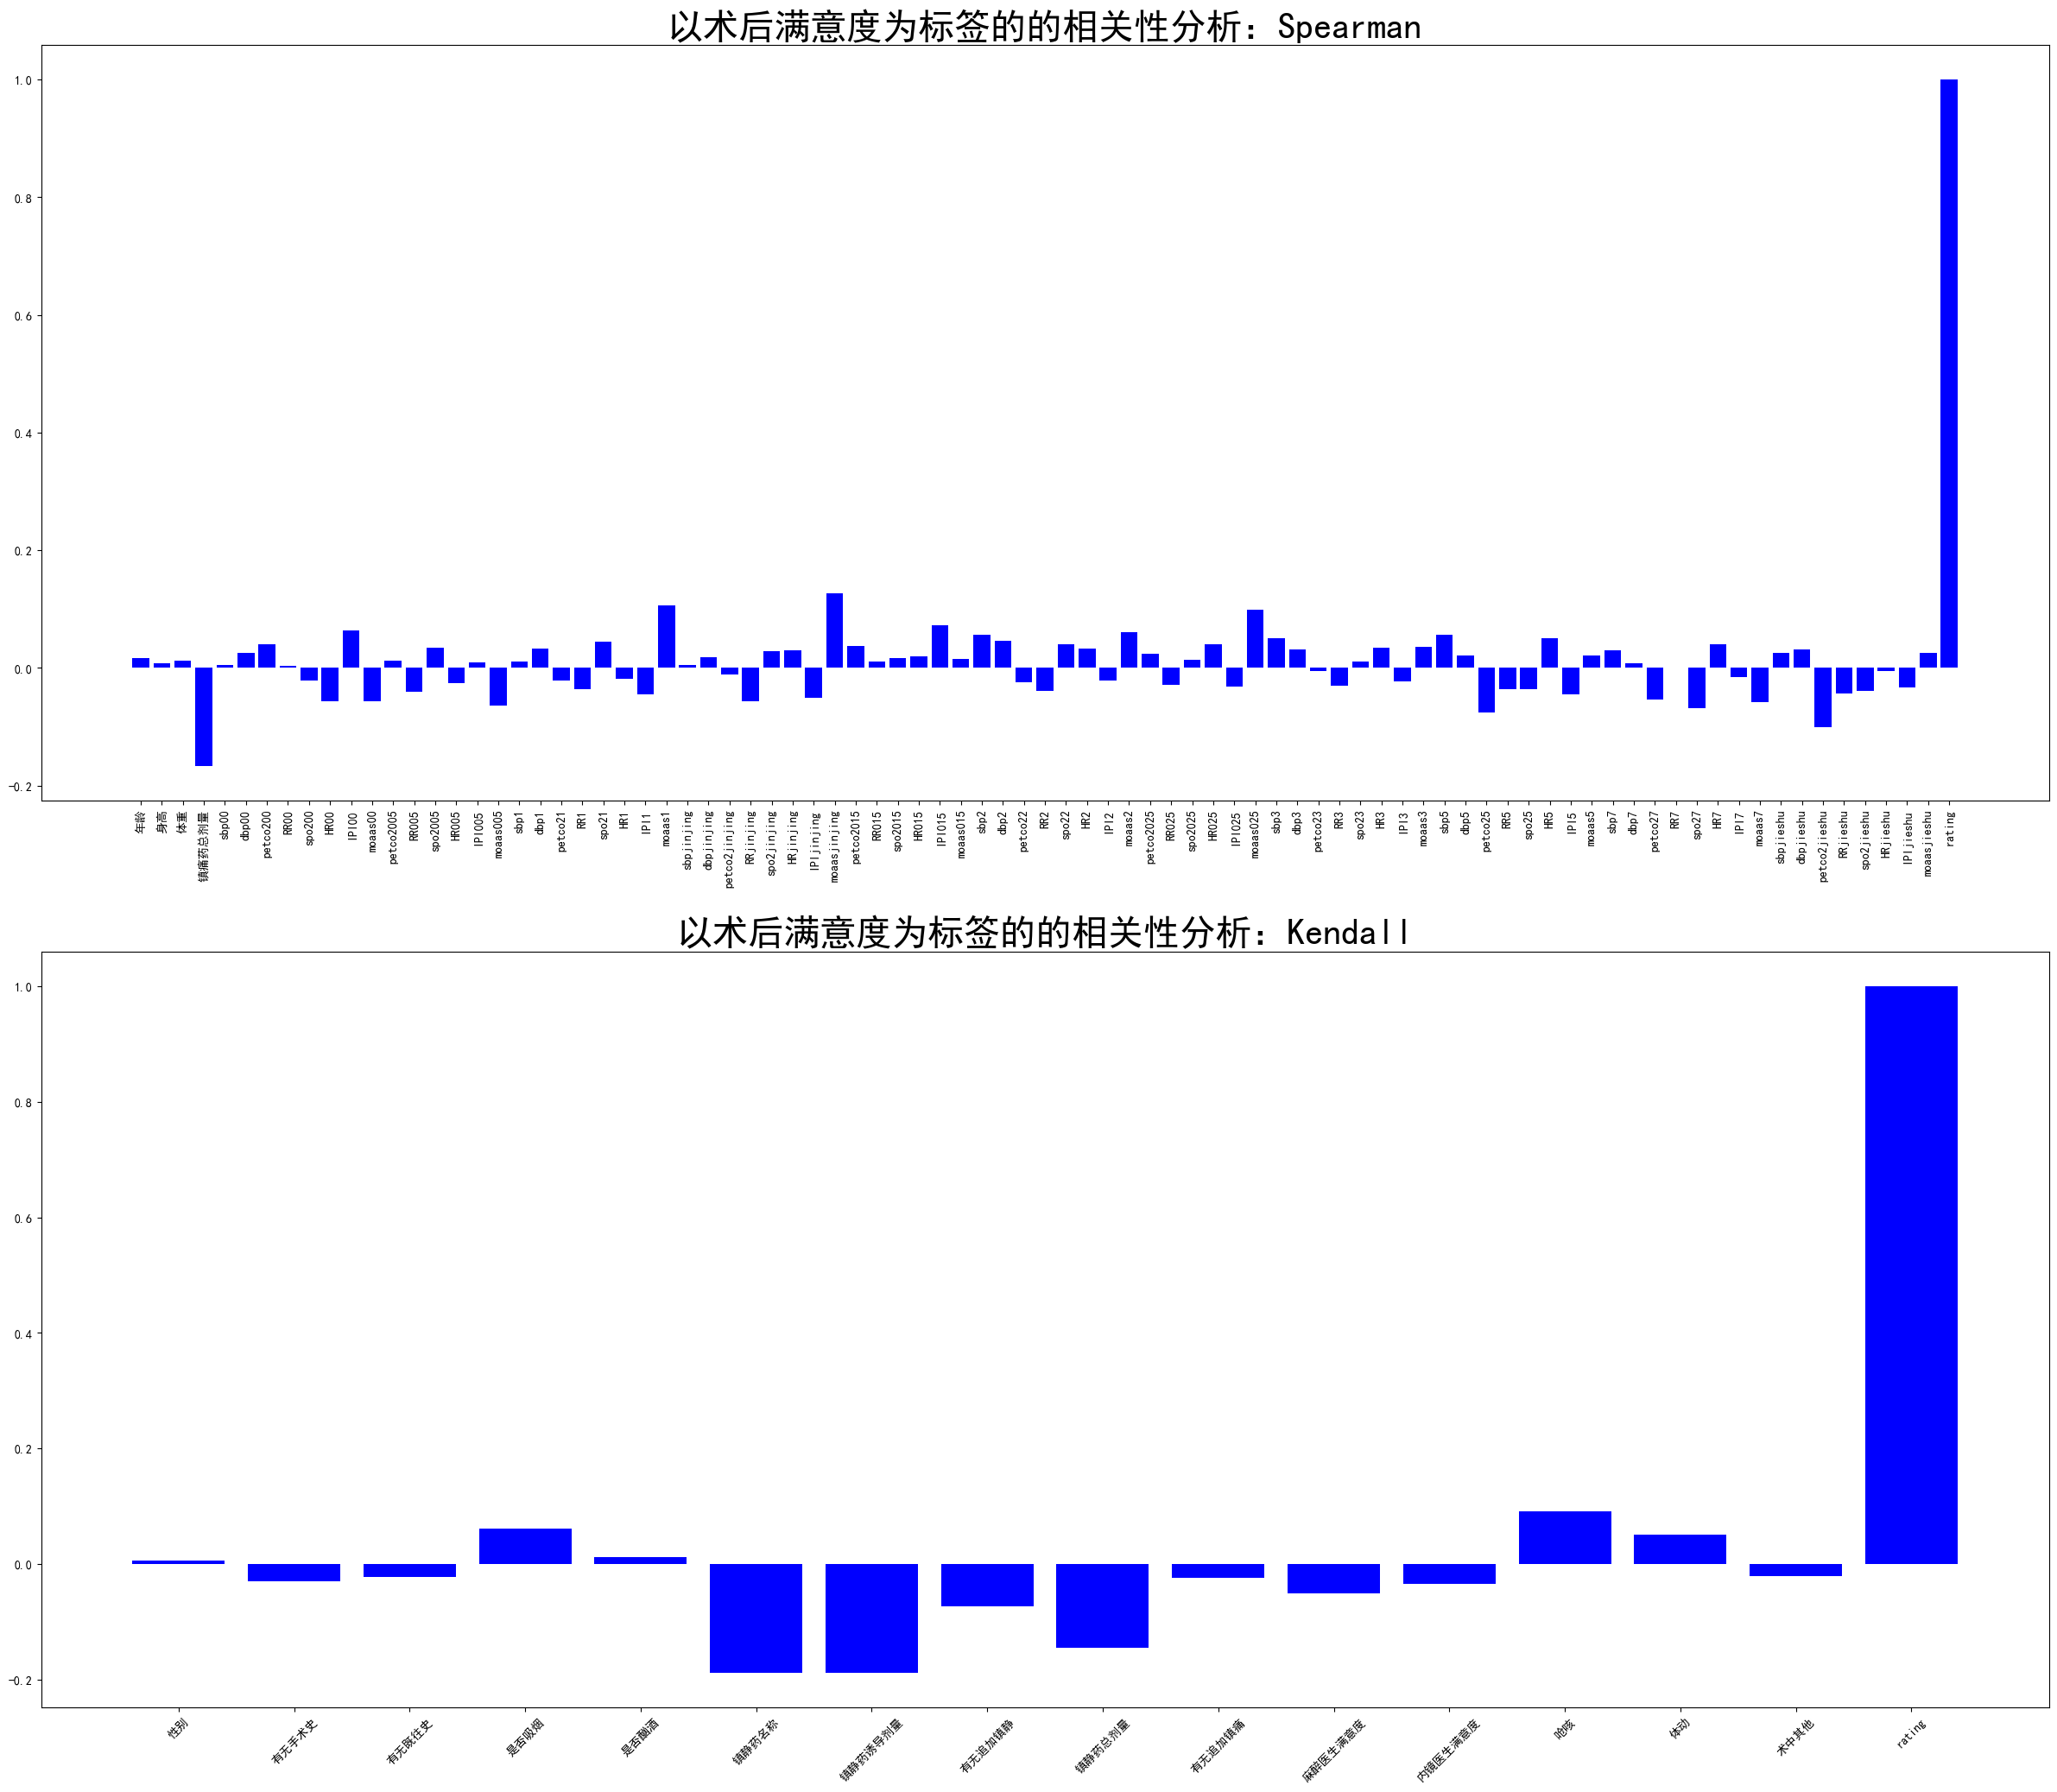
\includegraphics[width=0.95\textwidth]{10.png} 
	\label{Fig.main10} 
    \caption{以术后满意度为标签的相关性分析}
\end{figure}


由上图可知,第一个图展示的是使用Spearman相关性分析得到的各个特征与标签之间的相关系数,而第二个图展示的是使用Kendall方法得到的相关系数,条形图的x轴是各个特征的名称,y轴则是相应的相关系数。分析上图,由上分图关于数值型特征与术后满意度的Spearman相关系数得到相关性分析可以看出镇痛药的总剂量对于术后满意度的不良影响最大,这与现实情况是吻合的。而moaasjinjing与术后满意度的正向影响相关性最大,其中关于moaas的含量与术后满意的都有正相关性的关系,综合考虑,相关性的绝对值都不大于0.2。从统计学上分析存在的相关性并不大,但是相对而言镇痛药的对术后满意度的不良影响的相关性较大。由第二张图关于分类特征与术后满意度的Kendall相关性分析可以看出镇静药名称、镇静药诱导剂量、镇静药总剂量对于术后满意度的不良影响最大,而其他因素对于术后满意度的正向影响相关性都比较弱,综合考虑,相关性的绝对值都不大于0.2。从统计学上分析存在的相关性并不大,但是相对而言镇静药的名称、镇静药诱导剂量、镇静药总剂量对术后满意度的不良影响的相关性较大。综上,镇痛药和镇静药各种因素对于术后满意程度都有不利的影响,而moaas的含量对于术后满意度的影响是有利的。


通过这个图可以直观地比较不同特征与标签之间的相关性强度,但是由于术后满意度标签分布不均衡,可能会影响模型提取特征的效果,进而影响其准确率和稳定性,需要进一步优化模型。


\subsection{基于随机森林的分类标准挖掘}

为进一步探究出与术后满意度有关的因素,并挖掘出其间的定量关系,本文基于随机森林算法建立模型

\subsubsection{模型建立}

随机森林是一种集成学习方法,由多棵决策树组成。其公式可以分为两部分:随机森林的生成和随机森林的预测。随机森林的生成过程如下:

\begin{enumerate}
  \item 从原始数据集中采样出$n$个样本作为训练集,采用 bootstrap 技术进行采样,即每次从原始数据集中随机抽取一个样本并将其放回,重复$n$次得到大小为$n$的采样集。
  \item 从所有特征中随机选择$m$个特征,其中$m\ll d$,$d$为原始特征的总数。
  \item 利用上述采样得到的数据集和特征集构建一棵决策树,具体建树过程可以使用 ID3、C4.5 或 CART 等决策树算法。
  \item 重复步骤前三步$T$次,得到$T$棵决策树,这些决策树构成了随机森林。
\end{enumerate}
  
  
随机森林的预测步骤:

\begin{enumerate}
  \item 对于每个测试样本,对随机森林中的每棵决策树进行预测,得到预测结果。
  \item 对$T$个预测结果进行投票,将得票最多的类别作为随机森林的最终预测结果。
\end{enumerate}

随机森林的预测公式可以表示为:

\begin{equation}
    \widehat{y}=\arg {{\max }_{y}}\sum\limits_{i=1}^{T}{I\left( {{\widehat{y}}_{i}}=y \right)}.
\end{equation}
其中,$\widehat{y}$表示随机森林的预测结果,${{\widehat{y}}_{i}}$表示第$i$棵决策树的预测结果,$T$表示随机森林中的决策树数量,$y$表示所有可能的类别,$I(\cdot )$表示指示函数,当条件成立时取值为1,否则取值为 0。




\subsubsection{模型求解}

通过对标签进行分布分析,得出如下条形统计图:

\begin{figure}[H] % 这个H不要动!
	\centering % 不要动!
	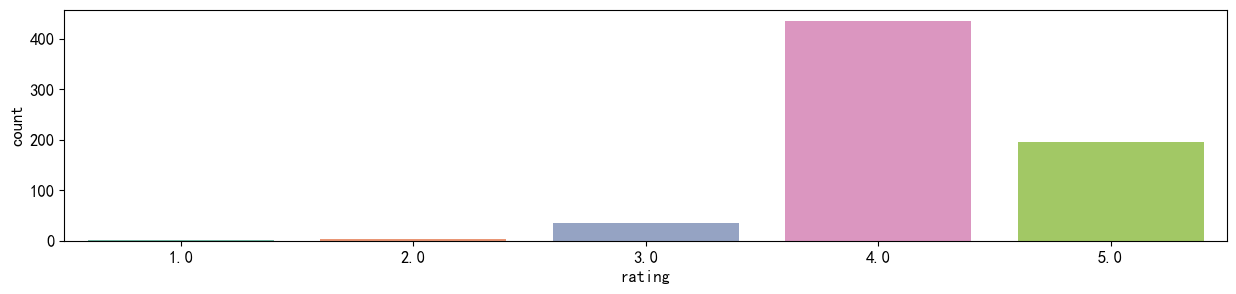
\includegraphics[width=0.95\textwidth]{11.png} 
	\label{Fig.main11} 
    \caption{术后24小时的分布分布图}
\end{figure}

通过上图可以看出,本次分类任务的数据集标签严重失衡,类似问题一中的处理,使用imblearn库中的RandomOverSampler方法对数据进行上采样,并将处理后的数据集分为训练集和测试集,其中测试集占比0.2,再用随机森林分类器进行训练和预测。基于Scikit-Learn将随机森林模型初始化,并使用训练集对其进行训练,最终分类器在测试集上的评估结果如下表所示:

\begin{table}[H]
    \centering  
    \caption{对随机森林的术后24小时满意度预测评价}
    \begin{tabular}{c c c c c}  
    	\toprule[1.5pt]  
    	类别 & 准确率 & 召回率 & F1分数 & 支持率 \\  
    	\midrule[1pt]    
        非常满意    & 0.56 & 0.60 & 0.58 & 97 \\ 
        满意        & 0.50 & 0.17 & 0.25 & 89 \\ 
        一般        & 0.61 & 1.00 & 0.76 & 76 \\ 
        不满意      & 0.95 & 1.00 & 0.98 & 83 \\ 
        非常不满意  & 1.00 & 1.00 & 1.00 & 91 \\ 
    	\toprule[1.5pt]  
    \end{tabular}  
\end{table} 

通过这个评价结果可以看出,该随机森林模型性能优良,预测结果可行度高。基于此背景,本文欲通过树模型独有的树状图探究分类的标准,从而了解与满意度有关的因素,并可以如题设所要求挖掘出具体的关系。通过plot\_tree函数导出max\_depth=3时的树状图如下:

\begin{figure}[H] % 这个H不要动!
	\centering % 不要动!
	\includegraphics[width=0.95\textwidth]{12.png} 
	\label{Fig.main12} 
    \caption{随机森林树状图导出}
\end{figure}

通过此图形,本文明确地得到:决策树所挖掘的数据内在的分类标准与每个特征指标之间存在的具体的数值关系,依据随机森林的原理,经过训练的树的每一层都会据特征空间的若干个特征进行分裂,从而模拟一种分类的效果。据图得到的结果如下:

\begin{table}[H]
    \centering  
    \caption{树状图信息挖掘}
    \begin{tabular}{c c c c c c}  
    	\toprule[1.5pt]  
    	层数 & 叶片编号 & 参考特征 & 分裂依据\\  
    	\midrule[1pt]    
    	1                  & 1     & petco2025     & petco2025$\leq 0.178$       \\ 
    
        \multirow{2}{*}{2} & 1-1   & RRjieshu      & RRjieshu$\leq 0.703$           \\
                           & 1-2   & petco2005     & petco2005$\leq 0.643$       \\
                           
        \multirow{4}{*}{3} & 1-1-1 & 镇静药总剂量  & 镇静药总剂量$\leq103.5$     \\
                           & 1-1-2 & RR2           & RR2$\leq0.241$              \\
                           & 1-2-1 & petco2005     & petco2005$\leq0.622$        \\
                           & 1-2-2 & sbp3          & sbp3$\leq0.296$             \\
    	\toprule[1.5pt]  
    \end{tabular}  
\end{table} 

通过上表可以看出树状图的每个叶片所蕴含的信息,关键的信息在于随机森林选取的叶片分裂的标准——这有助于本文建立术后满意度与影响因素的定量联系。通过该图可以得知,随机森林选取特征空间中的“petco2025”、“RRjieshu”、“petco2005”、“镇静药总剂量”、“RR2”、“petco2005”以及“sbp3”作为用于分类的特征,并按照严格的定量标准对每层叶片进行分裂。

然而从对随机森林的评价结果可以看出:尽管本文建立的随机森林模型在五分类任务整体准确率达到了0.75,然而从五个类别分别来看有两个类别正确率仅不足六成,故需考察底层叶片的具体信息,并通过Gini指数来严格判断给出的分类标准是否可信,以此来证明所建立的联系的严谨性,底层叶片信息如下:

\begin{table}[H]
    \centering  
    \caption{底层叶片的具体信息}
    \begin{tabular}{c c c c}  
    	\toprule[1.5pt]  
    	叶片编号  & 分裂结果  & Gini指数  & 主观可信度\\  
    	\midrule[1pt]
        1-1-1-1 &  \{0,0,172,198,215\}      & 0.664  & 差       \\
        1-1-1-2 &  \{0,238,92,55,28\}       & 0.596  & 差       \\
        1-1-2-1 &  \{0,0,0,7,4\}            & 0.463  & 良       \\
        1-1-2-2 &  \{0,115,0,0,0\}          & 0      & 优       \\
        1-2-1-1 &  \{0,0,28,13,27\}         & 0.636  & 差       \\
        1-2-1-2 &  \{345,0,0,1,2\}          & 0.017  & 优       \\
        1-2-2-1 &  \{0,0,47,25,19\}         & 0.614  & 差       \\
        1-2-2-2 &  \{0,0,21,48,44\}         & 0.633  & 差       \\
    	\toprule[1.5pt]  
    \end{tabular}  
\end{table} 

Gini指数是一种衡量节点纯度的指标,其体现的即为叶片分裂的可参考程度。对于五分类的随机森林模型,本文主观地根据八个底层叶片的Gini指数取值归类为“优”、“良”、“差”三类,舍弃对Gini指数表现较差的分类标准的参考,最终选取有效分类标准如下:

\begin{table}[H]
    \centering  
    \caption{有效联系挖掘}
    \begin{tabular}{c c c}  
    	\toprule[1.5pt]  
    	特征名称  & 分类标准  & 具体判别类别  \\  
    	\midrule[1pt]
        \multirow{3}{*}{分裂组1} & petco2025$\leq 0.178$ &  \multirow{3}{*}{“不满意”、“满意”、“非常满意”}    \\
                                 & RRjieshu$\leq  0.703$ &                                                   \\
                                 & RR2$\leq0.241$        &                                                   \\
        \multirow{3}{*}{分裂组2} & petco2025$\geq 0.178$ &  \multirow{3}{*}{“非常不满意”}                    \\
                                 & petco2005$\leq 0.643$ &                                                   \\
                                 & petco2005$\leq 0.622$ &                                                   \\ 
    	\toprule[1.5pt]  
    \end{tabular}  
\end{table}                

基于此表,关于各特征与术后满意度的联系尽收眼底,本文通过一个简易流程图来解释术后满意度与“petco2025”,“RRjieshu”,“RR2”,“petco2005”的联系:

\begin{figure}[H] % 这个H不要动!
	\centering % 不要动!
	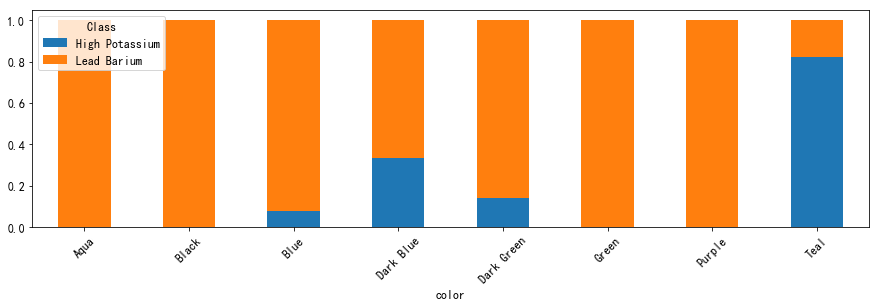
\includegraphics[width=0.95\textwidth]{15.png} 
	\caption{术后满意度与特征的定量联系} 
	\label{Fig.main15} 
\end{figure}
                       
这也进一步对分类的指标有了具体化的体现,说明上面的简单的相关性分析往往只能摸索出浅层次的结论,本文选用的随机森林算法具有深度挖掘类别与特征之间联系的能力,且具有推广价值。


















